%!TEX program = xelatex
\documentclass[12pt,a4paper]{article}
\usepackage{ctex}
\usepackage{amsmath,amscd,amsbsy,amssymb,latexsym,url,bm,amsthm}
\usepackage{epsfig,graphicx,subfigure}
\usepackage{enumitem,balance,mathtools}
\usepackage{wrapfig}
\usepackage{mathrsfs, euscript}
\usepackage[usenames]{xcolor}
\usepackage{hyperref}
%\usepackage{algorithm}
%\usepackage{algorithmic}
%\usepackage[vlined,ruled,commentsnumbered,linesnumbered]{algorithm2e}
\usepackage[ruled,lined,boxed,linesnumbered]{algorithm2e}

\newtheorem{theorem}{Theorem}[section]
\newtheorem{lemma}[theorem]{Lemma}
\newtheorem{proposition}[theorem]{Proposition}
\newtheorem{corollary}[theorem]{Corollary}
\newtheorem{exercise}{Exercise}[section]
\newtheorem*{solution}{Solution}

\renewcommand{\thefootnote}{\fnsymbol{footnote}}

\newcommand{\postscript}[2]
 {\setlength{\epsfxsize}{#2\hsize}
  \centerline{\epsfbox{#1}}}

\renewcommand{\baselinestretch}{1.0}

\setlength{\oddsidemargin}{-0.365in}
\setlength{\evensidemargin}{-0.365in}
\setlength{\topmargin}{-0.3in}
\setlength{\headheight}{0in}
\setlength{\headsep}{0in}
\setlength{\textheight}{10.1in}
\setlength{\textwidth}{7in}
\makeatletter \renewenvironment{proof}[1][Proof] {\par\pushQED{\qed}\normalfont\topsep6\p@\@plus6\p@\relax\trivlist\item[\hskip\labelsep\bfseries#1\@addpunct{.}]\ignorespaces}{\popQED\endtrivlist\@endpefalse} \makeatother
\makeatletter
\renewenvironment{solution}[1][Solution] {\par\pushQED{\qed}\normalfont\topsep6\p@\@plus6\p@\relax\trivlist\item[\hskip\labelsep\bfseries#1\@addpunct{.}]\ignorespaces}{\popQED\endtrivlist\@endpefalse} \makeatother
\begin{document}
\noindent

%========================================================================
\noindent\framebox[\linewidth]{\shortstack[c]{
\Large{\textbf{CS308 Homework 2}}\vspace{1mm}\\
Exercises for Algorithm Design and Analysis by Li Jiang, 2016 Autumn Semester}}
\begin{center}
\footnotesize{\color{blue} \quad Name:\underline{Gao Chao}  \quad Student ID:\underline {5142029014} \quad Email: \underline {gaoc96@163.com}}
\end{center}

\begin{description}
	\item[Coverage]: Syntax Analysis.
\end{description}

\begin{enumerate}
\item (Section 4.2, Exercises 4.2.1) Consider the context-free grammar:

    \begin{center}
    S $->$ S S + $|$ S S * $|$ a
    \end{center}
    
    and the string aa + a*.

    \begin{enumerate}
    \item Give a leftmost derivation for the string.
    \item Give a rightmost derivation for the string.
    \item Give a parse tree for the string.
    \end{enumerate}

\begin{solution}

%Your answer should be written here.
    \textrm{\\}
    \begin{enumerate}
    \item S $=>$ S S * $=>$ S S + S * $=>$ a S + S * $=>$ a a + S * $=>$ a a + a *
    \item S $=>$ S S * $=>$ S a * $=>$ S S + a* $=>$ S a + a *$=>$ a a + a *
    \item below is the parse tree

    \begin{figure}[h]
    \center
    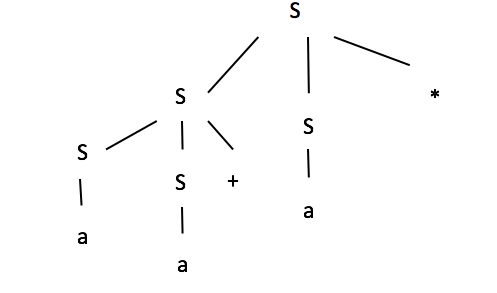
\includegraphics[width=0.8\linewidth]{sol}\vspace{-10pt}
    \caption{parse tree} \label{parse tree}\vspace{-10pt}
    \end{figure}
    \end{enumerate}

\end{solution}

\newpage
\textrm{\\}

\item (Section 4.3, Exercises 4.3.1) The following is a grammar for regular expressions over symbols $a$ and $b$ only, using + in place of $|$ for union, to avoid conflict with the use of vertical bar as a metasymbol in grammars:
    \begin{center}
    rexpr $->$ rexpr + rterm $|$ rterm
    
    rterm $->$ rterm rfactor $|$ rfactor
    
    rfactor $->$ rfactor * $|$ rprimary
    
    rprimary $->$ a $|$ b
    \end{center}

    \begin{enumerate}
    \item Left factor this grammar.
    \item Does left factoring make the grammar suitable for top-down parsing?
    \item In addition to left factoring, eliminate left recursion from the original grammar.
    \item Is the resulting grammar suitable for top-down parsing?
    \end{enumerate}

\begin{solution}
    \textrm{\\}
    \begin{enumerate}
    \item There is no common non-empty prefix, so we can't do left factoring, this grammar stays the same.
    \item No. Because this is the left-recursive grammar. If we use top-down parsing, it will get into an infinite loop.
    \item Below is the grammar after left recursion elimination.
    \begin{center}
    rexpr $->$ rterm A

    A $->$ + rterm A $|$ $\epsilon$
    
    rterm $->$ rfactor B

    B $->$ rfactor B $|$ $\epsilon$
    
    rfactor $->$ rprimary C
    
    C -> * C $|$ $\epsilon$

    rprimary $->$ a $|$ b
    \end{center}
    \item Yes. Because there is no left recursion.
    \end{enumerate}
%Your answer should be written here.

\end{solution}

\newpage
\textrm{\\}

\item (Section 4.4, Exercises 4.4.3) Compute FIRST and FOLLOW for the grammar:
    
        \begin{enumerate}
        \item S $->$ 0 S 1 $|$ 0 1 (with string 000111).
        \item S $->$ + S S $|$ * S S $|$ a (with string + * aaa).
        \end{enumerate}


\begin{solution}
    
    \textrm{\\}
    \begin{enumerate}
    \item FIRST(S) = [ 0 ],    FOLLOW(S) = [ 1, \$ ].
    \item FIRST(S) = [ +, *, a ],   FOLLOW(S) = [ +, *, a, \$ ].  
    \end{enumerate}
%Your answer should be written here.

\end{solution}

\end{enumerate}
%========================================================================
\end{document}